\documentclass{beamer}

\usepackage{graphicx}
\graphicspath{ {./images/} }

\usetheme{Madrid}
%\usetheme{Warsaw}

\title[Code]{Code in the Overlap project}

\author{R. Kuipers}

\begin{document}

\begin{frame}{General structure}
\begin{itemize}
\item Select mode
\item Read data from file
\item while not everything feasible
	\begin{itemize}
	\item Generate year model(year data, feedback)
	\item Solve year model
	\item Generate month data(year solution)
	\item for each month
		\begin{itemize}
		\item Generate month model(month data)
		\item Solve month model
		\item If feasible -$>$ next month
		\item Generate feedback model(month data)
		\item Solve feedback model	
		\end{itemize}
	\item double maxTime
	\end{itemize}
\end{itemize}
\end{frame}

\begin{frame}{Solving function}
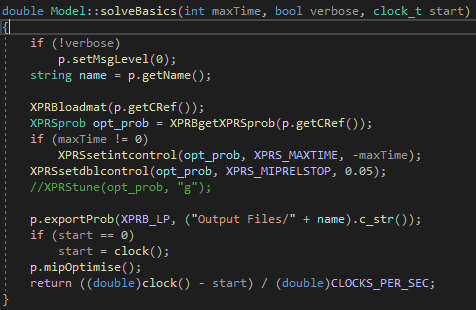
\includegraphics[width=\textwidth]{solve}
\end{frame}

\begin{frame}{Constraint generation}
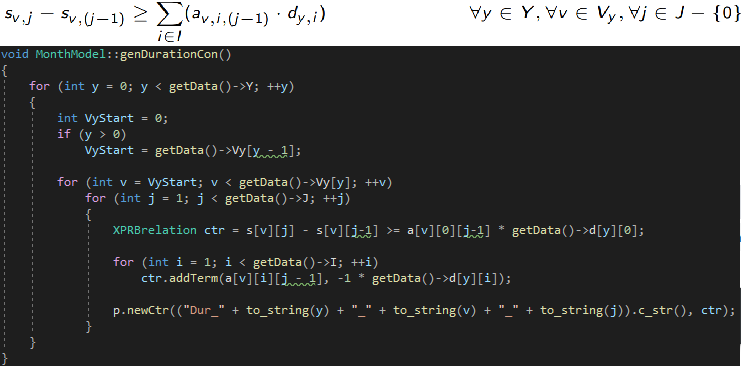
\includegraphics[width=\textwidth]{constraint}
\end{frame}

\begin{frame}{Splitting the problem up}
\begin{columns}
\begin{column}{0.33\textwidth}
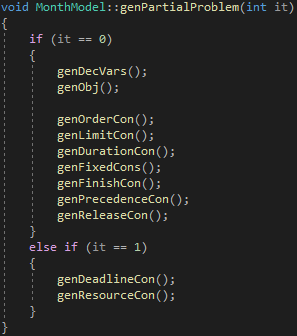
\includegraphics[width=\textwidth]{split1}
\end{column}
\begin{column}{0.66\textwidth}
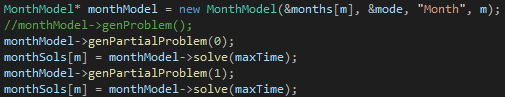
\includegraphics[width=\textwidth]{split2}
\end{column}
\end{columns}
\end{frame}

\begin{frame}{Feedback generation}
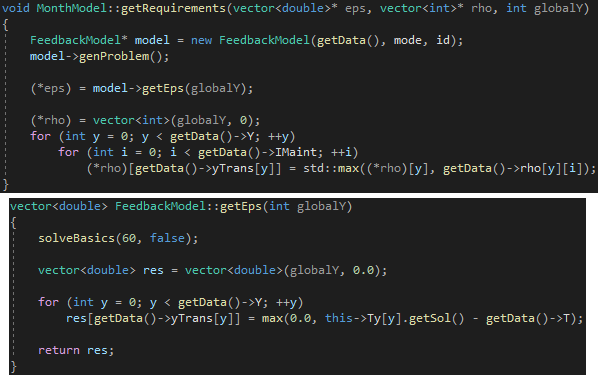
\includegraphics[width=\textwidth]{feedback}
\end{frame}

\begin{frame}{Ideas to try}
\begin{itemize}
\item Run program remotely on university PC (potentially faster, and can run in background)
\item Experiment more with splitting constraints
\item Improve feedback logic
\end{itemize}
\end{frame}

\end{document}


